\subsubsection{Leistungsfähigkeit bei unterschiedlichen Geschwindigkeiten}
%In diesem Abschnitt soll untersucht werden, ob eine Reduzierung der Geschwindigkeit positive Auswirkungen auf die Zuverlässigkeit von Bildverarbeitung und Regelung besitzt.

Nachdem eine passende Einstellung der Regel-und Bildverarbeitungsfrequenz gefunden wurde, soll nun das Fahren mit höheren Geschwindigkeiten betrachtet werden. Neben der normalen Sichtprüfung der Funktionalität der Fahrspurverfolgung wurden die Anzahl der zur Zielpunktbestimmung genutzten Weltkartenpunkte pro Regelung und der prozentuale Anteil an nicht bestimmten Zielpunkten zur Untersuchung herangezogen. 

Zur besseren Vergleichbarkeit der Messergebnisse wurden die Daten für je eine entgegen des Uhrzeigersinnes gefahrene Runde mit \SI{3}{\hertz} Bildverarbeitungsfrequenz aufgenommen.

\begin{figure}[h] % [htb]
	\centering
	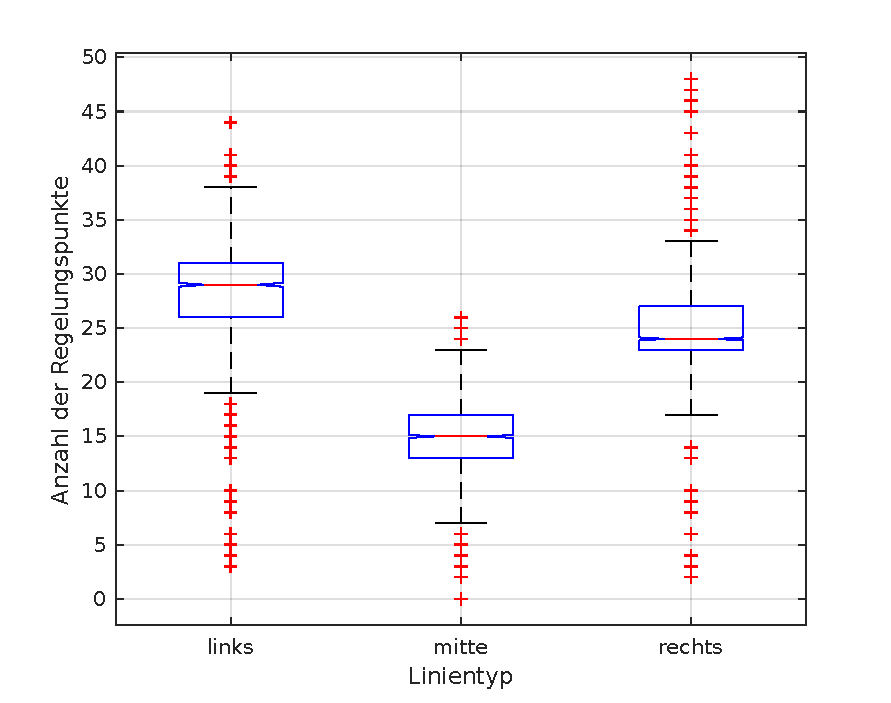
\includegraphics[width=0.9\textwidth]{evaluation_riverflow_regelungspunkte_je_linie_0.2m_s_3Hz.pdf}
	\caption{Anzahl der jeweiligen zur Regelung genutzten Punkte aus der Weltkarte bei \( \gls{lat:velocity} = \SI{0,2}{\metre\per\second} \)}
	\label{fig:evaluation:riverflow:regelungspunkte_je_linie}
\end{figure}

Abbildung~\ref{fig:evaluation:riverflow:regelungspunkte_je_linie} zeigt exemplarisch für die Geschwindigkeit \( \gls{lat:velocity} = \SI{0,2}{\metre\per\second} \) den  Anteil jeweiliger Linienpunkttypen zur Zielpunktberechnung. Es fällt sogleich auf, dass die Mittellinie einen weniger starken Einfluss nimmt. Da pro Strich und Bild nur ein Punkt in der Weltkarte eingetragen wird, ist deren Punkteanzahl geringer. Wie unter \ref{item:regelung:zielpunkt:holen:regeln:xcoord} in Kapitel \ref{ssec:regelung:zielpunkt:holen} beschrieben, werden die Regelungspunkte unter anderem nach ihrer x-Koordinate ausgewählt. In einer Linkskurve fallen dadurch mehr Punkte der linken Randlinie in das Suchfenster. Da die Strecke in der befahrenen Richtung vorrangig Linkskurven aufweist, werden im Mittel mehr linke als rechte Randpunkte zur Zielpunktberechung herangezogen.

\begin{figure}[h] % [htb]
	\centering
	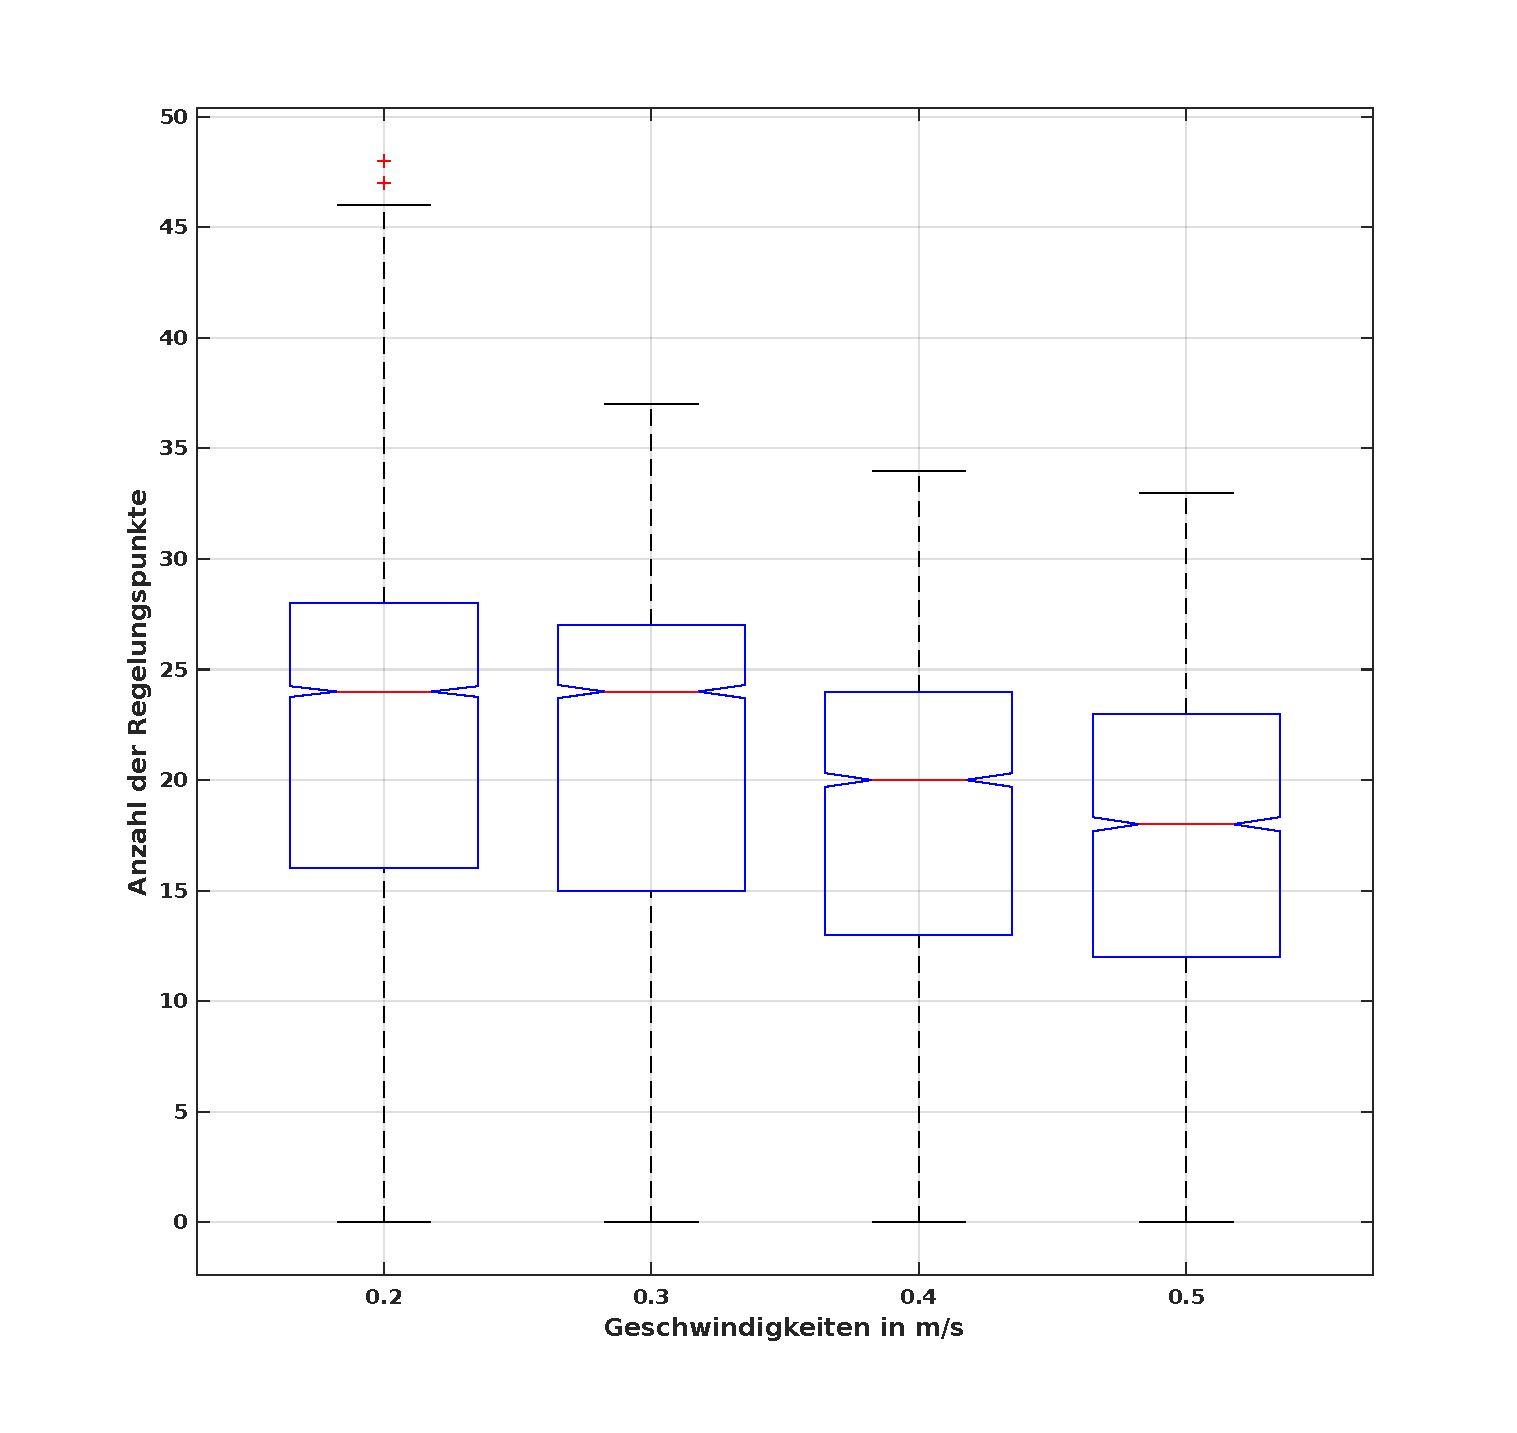
\includegraphics[width=0.9\textwidth]{evaluation_riverflow_regelungspunkte_je_geschw_3Hz.pdf}
	\caption{Anzahl der zur Regelung verwendeten Kartenpunkte zu verschiedenen Geschwindigkeiten}
	\label{fig:evaluation:riverflow:regelungspunkte_je_geschw}
\end{figure}

Betrachten wir die Gesamtzahl der zur Regelung verwendeten Punkte, ist wie in Abbildung~\ref{fig:evaluation:riverflow:regelungspunkte_je_geschw} ein Abfallen der Anzahl mit ansteigender Geschwindigkeit des Fahrzeugs zu beobachten. Wenn das Auto schneller fährt, liegt ein Punkt in der Karte umso eher außerhalb des Bereiches, aus dem die Regelungspunkte genutzt werden. Bei gleichbleibender Bildfrequenz wird zwischen jedem Bild eine größere Strecke zurückgelegt, sodass die Dichte der Weltkartenpunkte geringer wird. Der dargestellte Boxplot erfüllt also die Erwartungen.

Die mit unserer Implementierung erreichbare Höchstgeschwindigkeit sollte folglich dann erreicht sein, wenn der mobile Roboter fast ausschließlich nach den Informationen eines Bildes regelt oder sogar zwischenzeitlich keine Zielpunkte mangels Regelungspunkte bestimmen kann. Mit anderen Worten: Wenn sich das Auto zwischen zwei Fotoaufnahmen bis zum Sichtende des ersten Bildes bewegt, wie der Riverflow-Algorithmus Punkte erkennen konnte, ist die Maximalgeschwindigkeit beinahe erreicht. Ein Indiz dafür ist neben der visuellen Auffälligkeit des Fahrspurverlasses die starke Zunahme der nicht gefundenen Zielpunkte. 

\begin{figure}[h] % [htb]
	\centering
	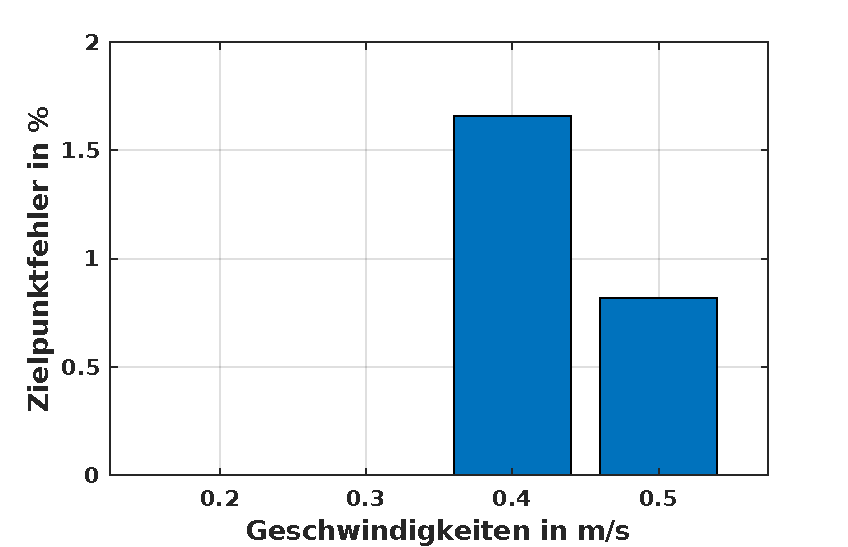
\includegraphics[width=0.9\textwidth]{evaluation_riverflow_zielpunktfehler_je_geschw_3Hz.pdf}
	\caption{Anteil der unbestimmten Zielpunkte einer Runde auf dem Parcours mit verschiedenen Geschwindigkeiten}
	\label{fig:evaluation:riverflow:zielpunktfehler_je_geschw}
\end{figure}

Was in Abbildung~\ref{fig:evaluation:riverflow:zielpunktfehler_je_geschw} zu sehen ist, war ebenfalls während des Fahrversuches am Auto zu beobachten. Ab einer Geschwindigkeit von \( \gls{lat:velocity} = \SI{0,4}{\metre\per\second} \) fuhr das Fahrzeug instabiler und die Latenzzeit der Regelung war dahingehend zu bemerken, dass in Kurven meist etwas zu spät und kurz darauf zur Korrektur zu viel eingelenkt wurde. Dies führte zu einer schwingenden Fahrweise (das Auto fuhr \glqq Schlängellinien\grqq). 

Die begrenzende Komponente für die Geschwindigkeit ist hier allerdings nicht zwingend die Bildfrequenz, sondern das Getriebe. Durch dessen kurze Übersetzung beträgt die Geschwindigkeit im Maximum 4500 tics pro Sekunde, was in etwa \SI{0,43}{\metre\per\second} entspricht. Die im Plot bezeichneten \SI{0,5}{\metre\per\second} dürften folglich nicht genau stimmen, auch wenn dies der eingestellte Wert des Geschwindigkeitsparameters war. Sie geben die Daten zu der dem ersten Auto maximal physikalisch möglichen Geschwindigkeit an. 

Ergänzend muss hier erwähnt werden, dass bereits ein zweites Fahrzeug mit ca. doppelt so langer Übersetzung existiert. Jedoch misslang eine Testfahrt mit unveränderten Parametereinstellungen bei höheren Geschwindigkeiten. Auch hier zeigte sich die Grenze an der \SI{0,5}{\metre\per\second}-Marke.

